\qquad 
TLS全称“Transport Layer Security(安全传输层)”,用于在两个通信应用程序之间提供保密性和数据完整性,常用于Web应用中客户端与服务器的加密通信。虽然TLS协议被定义为传输层的安全协议,但实际在抓包结果中可以看到TLS协议部分是被封装在TCP等传输层协议内的,而应用层的内容则封装在TLS内。在登录西安交通大学学生版统一认证网关的过程中,客户端页面也采用TLS加密方式向服务器提交表单,因此通过本实验也能对西安交通大学统一认证网关的安全机制有更好的了解。\\
\qquad
通过查阅国内相关文献 \cite{TLS-1} 以及国外的一些文献 \cite{TLS-2} ,可以了解到TLS协议由记录协议、更改密码协议以及警告协议三个高层协议构成,其中,记录协议还包括握手子协议。记录协议从高层ssL子协议收到数据后,对它们进行数据分段、压缩、认证和加密形成ssL记录;更改密码规格协议将密文状态由挂起状态复制到当前状态;警告协议用来传递ssL的相关警告。由于握手过程是可以被Wireshark软件轻易捕获的,在抓包时,我们主要关心的是TLS协议中的握手过程。TLS的握手过程如图 \ref{fig1} 所示。\\
\begin{figure}
	\centering
	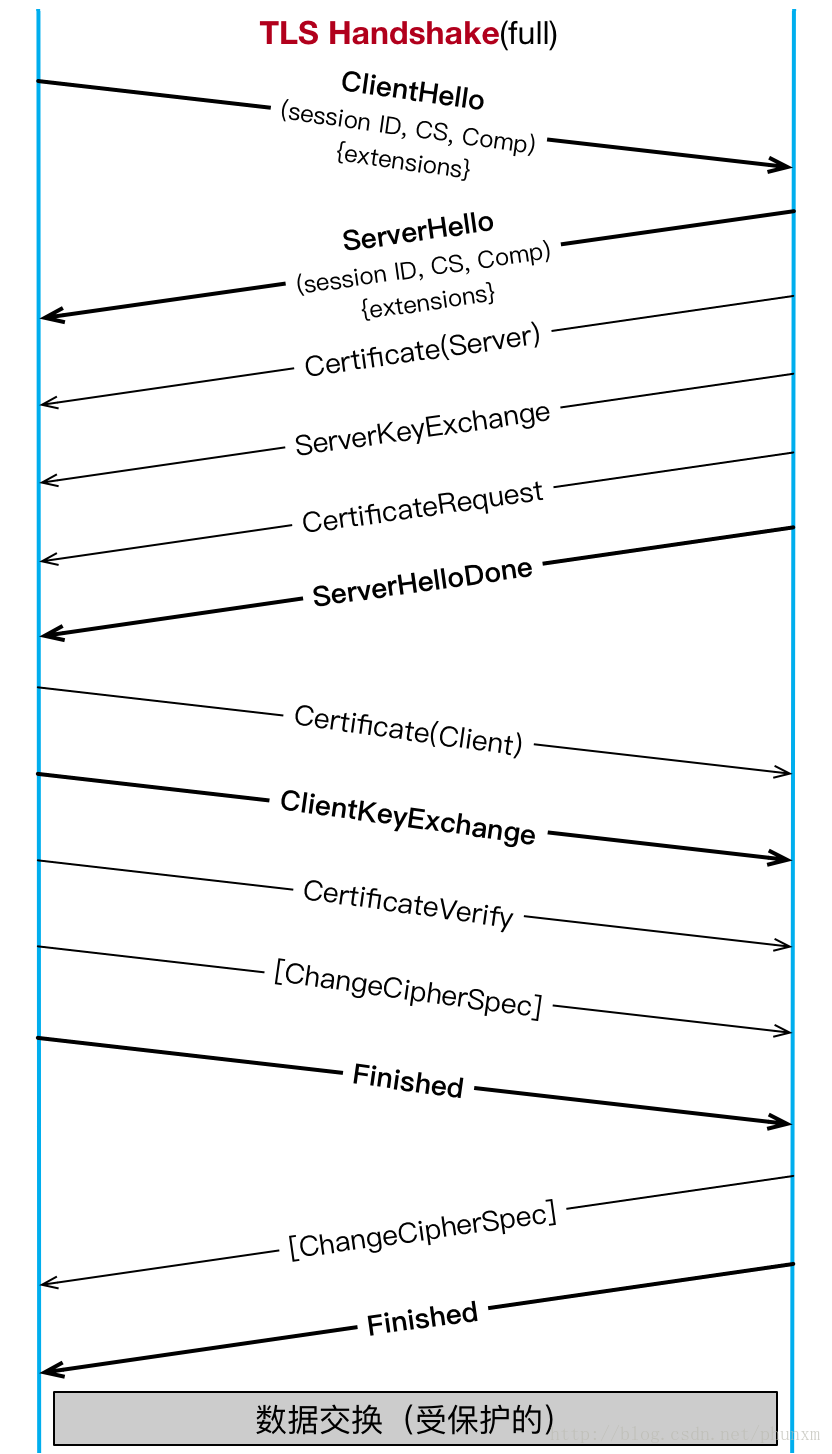
\includegraphics[width=8cm]{image/TLS-Handshake}
	\caption{TLS协议握手过程 \cite{TLS-3}}
	\label{fig1}
\end{figure}
\qquad
在图 \ref{fig1} 中,左侧代表客户端,右侧代表服务端。当客户端向服务端发起握手时,客户端首先向服务端发送“ClientHello”字段,包含会话ID(Session ID)等信息;服务端收到“ClientHello”字段后,返回一个“ServerHello”字段,同样包含会话ID等信息;之后服务端和客户端之间会进行密钥交换,在结束握手前,客户端和服务器还向依次向对方发送更改密钥的信息。\\
\qquad
但在实际的网络应用中,TLS协议的握手过程是否真的如图 \ref{fig1} 所示。本实验将通过Wireshark软件对西安交通大学学生版统一身份认证网关的登录过程进行抓包分析,以探究竟。\\